\documentclass[tikz,border=4pt]{standalone}
\usepackage{ctex}\usepackage{pgfplots}\pgfplotsset{compat=1.18}
\begin{document}
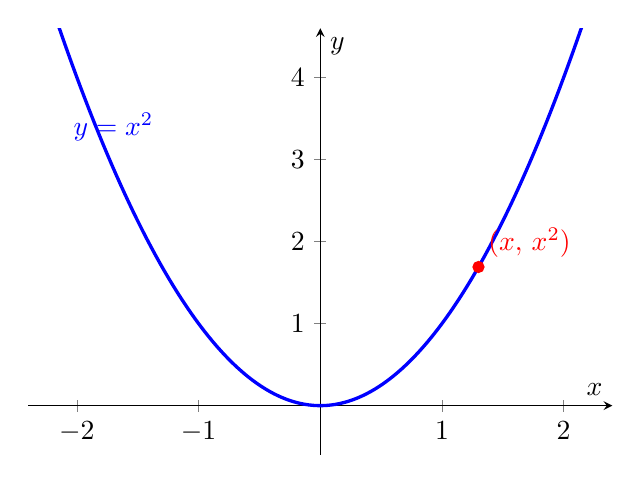
\begin{tikzpicture}
\begin{axis}[axis lines=middle,xlabel={$x$},ylabel={$y$},xmin=-2.4,xmax=2.4,ymin=-0.6,ymax=4.6,width=9cm,height=7cm,xtick={-2,-1,1,2},ytick={1,2,3,4},samples=120]
\addplot[blue,very thick,domain=-2.15:2.15]{x^2};
\addplot[only marks,red,mark=*] coordinates{(1.3,1.69)};
\node[red,anchor=south west] at (axis cs:1.3,1.69){$(x,\,x^2)$};
\node[blue] at (axis cs:-1.7,3.4){$y=x^2$};
\end{axis}
\end{tikzpicture}
\end{document}
